\documentclass[12pt, a4paper]{article}
\usepackage[francais]{babel}
\usepackage{caption}
\usepackage{graphicx}
\usepackage[T1]{fontenc}
\usepackage{listings}
\usepackage{geometry}
\usepackage[colorlinks=true,linkcolor=black,anchorcolor=black,citecolor=black,filecolor=black,menucolor=black,runcolor=black,urlcolor=black]{hyperref}

% \usepackage{mathpazo} --> Police à utiliser lors de rapports plus sérieux

\usepackage{fancyhdr}
\pagestyle{fancy}
\lhead{}
\rhead{}
\chead{}
\rfoot{\thepage}
\lfoot{Martin Baumgaertner}
\cfoot{}

\renewcommand{\headrulewidth}{0.4pt}
\renewcommand{\footrulewidth}{0.4pt}

\begin{document}
\begin{titlepage}
	\newcommand{\HRule}{\rule{\linewidth}{0.5mm}} 
	\center 
	\textsc{\LARGE iut de colmar}\\[6.5cm] 
	\textsc{\Large R401 -- Infrastructure de sécurité}\\[0.5cm] 
	\textsc{\large Année 2022-23}\\[0.5cm]
	\HRule\\[0.75cm]
	{\huge\bfseries TP1/2 - Chiffrement et TLS}\\[0.4cm]
	\HRule\\[1.5cm]
	\textsc{\large martin baumgaertner}\\[6cm] 

	\vfill\vfill\vfill
	{\large\today} 
	\vfill
\end{titlepage}
\newpage
\tableofcontents
\newpage
\section{TP1 - Chiffrement et PKI}
\subsection{Chiffrement}
    \subsubsection{Permutation}
    \subsubsection*{Question 1}
    Le message déchiffré que j'obtiens est \texttt{MAITRE CORBEAU SUR UN ARBRE PERCHEX}
    Voici ce que j'ai fait pour obtenir ce message :
    \begin{enumerate}
        \item J'ai créé une liste des lettres de l'alphabet, dans l'ordre.
        \item J'ai créé une deuxième liste, contenant les nombres 1 à 6.
        \item J'ai apparié les lettres et les chiffres des deux listes, dans l'ordre spécifié dans la clé.
        \item J'ai utilisé les chiffres pour créer une nouvelle séquence de lettres, en remplaçant chaque lettre du message d'origine par la lettre qui lui correspond dans la nouvelle séquence.
        \item J'ai supprimé tous les espaces de la chaîne obtenue.
    \end{enumerate}

    \subsubsection{Substitution}
    \subsubsection*{Question 2}
    Voici le message que j'ai trouvé \texttt{UN SECRET}

    \subsubsection{Diffie-Hellman}
    \subsubsection*{Question 3}
    J'ai obtenu \texttt{K = 117}

    \subsubsection{Chiffrement symétrique AES}
    \subsubsection*{Question 5}
    Voici le résultat que l'on obtient en base64 : \\

    \texttt{U2FsdGVkX1+QhnAugHjdc6bhMEMibXxWGQSE6ZKN56o=,}\\

    L’option “-nosalt” lors d’une commande openssl permet de ne pas rajouter de valeur aléatoire au code avant son hachage. En effet “salt” rajoute une valeur aléatoire pour renforcer le code/mot de passe.

    \newpage
    \subsection{PKI}   
    \subsubsection{Création du Certificat Racine (ou CA) et de sa clé privée.}
    \textbf{CA} signigie \textbf{C}ertificate \textbf{A}uthority. C'est une entité qui émet des certificats numériques.\\

    \subsubsection{Lecture du certificat}
    Ci-dessous, un tableau avec les différents \textbf{champs}
    et \textbf{fonctions} du certificat.
    \begin{center}
        \begin{tabular}{|c|c|}
            \hline
            \textbf{Champ} & \textbf{Fonction} \\
            \hline
            Version & Version du certificat \\
            \hline
            Serial Number & Numéro de série du certificat \\
            \hline
            Signature Algorithm & Algorithme de signature \\
            \hline
            Issuer & Entité qui a signé le certificat \\
            \hline
            Validity & Période de validité du certificat \\
            \hline
            Subject & Entité à qui le certificat est destiné \\
            \hline
            Subject Public Key Info & Informations sur la clé publique \\
            \hline
            X509v3 extensions & Extensions du certificat \\
            \hline
        \end{tabular}
    \end{center}

    \subsubsection{Contenu du CSR}
    \textbf{CSR} signifie \textbf{C}ertificate \textbf{S}igning \textbf{R}equest. C'est une requête de signature de certificat.\\
    Voici ci-dessous un tableau listant les \textbf{champs} et \textbf{fonctions} du CSR.
    \begin{center}
        \begin{tabular}{|c|c|}
            \hline
            \textbf{Champ} & \textbf{Fonction} \\
            \hline
            Version & Version du CSR \\
            \hline
            Subject & Entité à qui le certificat est destiné \\
            \hline
            Subject Public Key Info & Informations sur la clé publique \\
            \hline
            X509v3 extensions & Extensions du certificat \\
            \hline
        \end{tabular}
    \end{center}

    \subsubsection{Création de la liste de révocation}
    \textbf{CRL} signifie \textbf{C}ertificate \textbf{R}evocation \textbf{L}ist. C'est une liste de révocation de certificats.\\


\newpage
\section{TP2 - TLS Authentification}
\subsection{Openssl}
\subsubsection{Openssl et firefox}
\subsubsection*{Question 1}
Pour eviter d'avoir des messages d'erreurs et pour que firefox accepte de se connecter au serveur
sans rajouter des exception de sécurité, il faut :\\

\begin{itemize}
    \item que le certificat du serveur soit signé par une autorité de certification reconnue par firefox.
    \item correctement configurer le serveur web en utilisant le port HTTPS (443)
\end{itemize}

\subsubsection*{Question 2}
L'interface sur laquelle  est faite la capture dépend de notre machine sur la mienne il 
s'agit de l'interface nommée \texttt{eth0}.\\
Le filtre utilisé afficher les paquets propre à \textbf{TLS} est tout simplement le filtre 
\texttt{tls}.

\subsubsection*{Question 4}
Ci après le schéma du handshake du protocole TLS1.2 entre le client et le serveur: 

\begin{figure}[h]
    \centering
    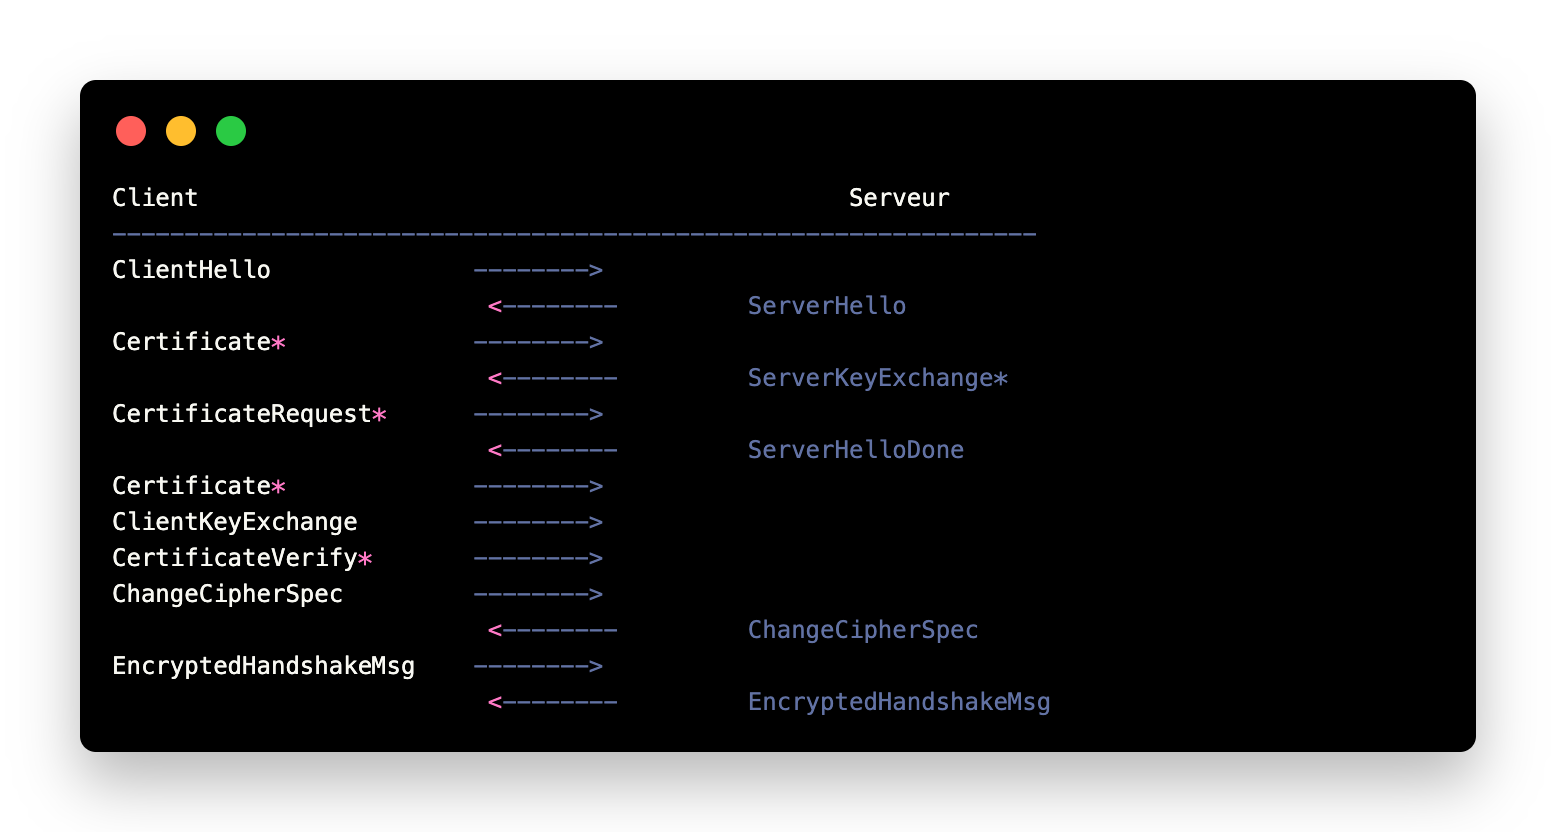
\includegraphics[width=0.9\textwidth]{img/handshake.png}
    \caption{Handshake TLS1.2}
    \label{fig:handshake}
\end{figure}

\subsection{Vérification OCSP}
\subsubsection*{Question 5}
L'erreur remontée par le navigateur indique que le certificat est révoqué. 

\subsubsection*{Question 6}
Une fois avoir exporté l'index des certificats et en relançant le responder OCSP nous avons 
bien la page internet qui s'affiche. 

\subsection{Vérification OCSP stapling}
\subsubsection*{Question 7}
Non, cela ne règle pas les problèmes de latence et de confidentialité. Cette variante 
d'OCSP permet au serveur web de fournir la réponse de vérification dans un nouveau 
message du Handshake, elle ne règle pas les problèmes inhérents à OCSP. Ces limitations ont conduit les navigateurs 
modernes à désactiver la vérification OCSP par défaut pour améliorer l'expérience 
utilisateur.

\subsection{Apache}
\subsubsection*{Question 9}
Pour utiliser mes certificats j'ai du indiqué l'emplacement de mon certificat finissant par
l'extension \textbf{.crt} dans le fichier \textbf{default-ssl.conf}, à la ligne 
\textbf{SSLCertificateFile}. Et, à la ligne \textbf{SSLCertificateKeyFile} j'ai dû indiquer
l'emplacement de ma clé privé.\\

Voici donc les lignes : 
\begin{itemize}
    \item \texttt{SSLCertificateFile /etc/ssl/mondomaine/mondomaine.crt}
    \item \texttt{SSLCertificateKeyFile /etc/ssl/mondomaine/mondomaine.key}\\
\end{itemize}

Il ne faut pas oublier de rédemarrer Apache pour les modifications soient prises en 
compte avec la commande \texttt{sudo service apache2 restart}

\end{document}